\documentclass{article}
\usepackage{rotating}
\usepackage{verbatim}
\usepackage{graphicx}

\begin{document}

\title{Surfpack Version 1.0 (beta) User's Manual}

\author{Anthony A. Giunta, Mark D. Richards, Eric C. Cyr \\Laura P. Swiler, Shane L. Brown, Michael S. Eldred}

\maketitle

\pagebreak

\section {Overview}\label{sec:overview}
Surfpack is a collection of surface-fitting methods and accompanying metrics to evaluate or predict the quality of the generated surfaces.  The concept of creating a global approximation or ``fit'' from a collection of data samples is utilized in many scientific disciplines, but the nomenclature varies widely from field to field.  The results from the application of such methods are commonly called empirical models, response surfaces, surrogate models, function approximations, or neural networks.  Many different algorithms have been developed to generalize from a set of data; these algorithms have different strengths and weaknesses.  The goals of Surfpack are

\begin{enumerate}
\item to give users the option to use any of several methods, depending on the nature of the specific application; and
\item to put data-fitting methods that are commonly used in various disciplines into a common framework, where their properties can be more easily compared and analyzed.
\end{enumerate}
Surfpack's API includes a small set of commands, centered on the following general operations:
\begin{itemize}
\item {\bf Prepare a data set for use.}  This typically involves reading a formatted text file from disk.  Alternatively, the user may specify upper- and lower-bounds along one or more dimensions and generate a set of data points from those boundaries (either a grid or a set of Monte Carlo samples).
\item {\bf Create an empirical model from a set of data.} The user may choose one of several algorithms to create the surface approximation: Least-squares regression using polynomials, Multivariate Adaptive Regression Splines (MARS), Kriging interpolation, Artificial Neural Networks, or Radial Basis Function Networks.
\item {\bf Evaluate an empirical model on a set of data.}  For the non-interpolating algorithms (e.g. polynomial regression), it may be of interest to evaluate the model at the same data sites that were used to generate it, to see how closely the model fits the data.  All of the algorithms all the user to evaluate the model at other data points where the true function value is not available.
\item {\bf Obtain measures of the ``goodness of fit'' of the model.}  Surfpack supports metrics such as mean squared error or maximum absolute error for data sets where the true function values are known.  Cross-validation metrics (e.g. PRESS) are also available for situations where all of the known data points for the function that is being approximated were used to create the empirical model.
\item {\bf Save the data and/or empirical models for future use.}  Data can be saved for later use, e.g., with a plotting package.  The approximating surfaces themselves may also be saved, so that a user can evaluate the model on a data set at a later time without having to recompute it.
\end{itemize}


\section{Installation}\label{sec:installation}
Surfpack is being developed primarily under Linux and is targeted to all flavors of UNIX.  Platforms on which Surfpack has been successfully built include Linux, SunOS, IRIX, OSF, and AIX.  Surfpack does not currently build under Windows or Mac OS X; these may be supported in future releases.
\subsection{Requirements}
\begin{itemize}
\item C++.  A majority of the source code for Surfpack is written in C++.  Surfpack makes heavy use of the standard C and C++ libraries, including the standard template libraries.
\item Fortran 77.  The MARS and Kriging algorithms are implemented in Fortran.  The Kriging algorithm uses the constrained optimizer CONMIN, which is also written in Fortran.  
\item BLAS.  Many of the data-fitting algorithms rely on the Basic Linear Algebra routines to perform rudimentary linear algebra operations.
\item LAPACK.  Surfpack makes use of the following LAPACK driver routines: dgetrf, dgetri, dgels, dgglse.  Implementations of LAPACK across different platforms seem to vary in terms of how many of these algorithms they support.  Therefore, source for these functions and there dependences is included in the Surfpack distribution.  However, BLAS and LAPACK routines are usually heavily optimized for each platform; performance is likely to be best if pre-compiled, native versions of these functions are available.
\end{itemize}
\subsection{Options}
\begin{itemize}
\item CPP Unit.  A suite of unit tests is available on platforms where CPP Unit has been built.
\item Flex and Bison. Surfpack may be used as a library or as a stand-alone program.  The stand-alone executable requires Flex and Bison (a lexical analyzer generator and parser generator, respectively), which are freely available on the Internet.
\end{itemize}
\subsection{Standard build}
The Surfpack build system uses the GNU autotools: autoconf, automake, and libtool.  The autotools do not need to be installed to build Surfpack, but they should be used by developers who wish to extend Surfpack.  To build Surfpack from source, first obtain the distribution tarball surfpack-0.1.tar.gz.  From the directory containing this file, execute the following commands:
\begin{enumerate}
\item gunzip surfpack-0.1.tar.gz
\item tar xf surfpack-0.1.tar
\item cd surfpack-0.1
\item ./configure
\item make
\item make install
\end{enumerate}

Users with access to Surfpack's CVS respository may checkout the source directly instead of downloading the gzipped distribution tar-file.  In this case, the user must manually run the GNU autotools to create the configure script and Makefile.in files.  The appropriate sequence of commands would be
\begin{enumerate}
\item cvs checkout Surfpack
\item cd Surfpack
\item autoreconf --install
\item items 4--6 above
\end{enumerate}
By default, the Surfpack library is installed in /usr/local/lib.  If appropriate Flex and Bison distributions are available, the stand-alone executable, named \texttt{surfpack}, will be be installed in /usr/local/bin.  Adding files to these directories generally requires super-user privileges.  To install Surfpack in another location, use the --prefix option to configure.  For example, the command

\texttt{./configure --prefix=/home/userid}

would lead to the installation of the Surfpack library and executable as /home/userid/lib/libsurfpack.a and /home/userid/bin/surfpack respectively. If these files are not present at the conclusion of the build, see section xx for installation troubleshooting tips.
\subsection{Advanced options}
Most deviations from the standard build process involve special arguments to configure.
\subsection{Testing the installation}
Surfpack is distributed with its test suite.  The unit testing suite utilizes the CPP Unit libraries, available at <URL>, which must be installed in the users's machine if the tests are to be executed.  If the CPP Unit libraries are installed in a location that is not automatically searched by the compiler, the full path of the libraries should be specified as an argument to configure:
\texttt{./configure --with-cppunit-prefix=/home/userid/cppunit}
To run the test suite, type \texttt{make check} at the command line, after the successful execution of \texttt{make} or \texttt{make install}.  CPP Unit summarize the results of the tests.

If Surfpack is built as a stand-alone executable (as it is by default), additional tests are available in the examples subdirectory.

\subsubsection{Specifying your compiler}
By default, configure will use the first available C++ compiler from the following list: xlC, CC, cxx, c++, g++.  To override this selection process, use the CXX option.  The command

\texttt{./configure CXX=g++}

will cause g++ to be used, regardless of the presence of any other C++ compilers.  Likewise, the default search order for a Fortran 77 compiler is xlf, f77, g77.  To override the default, use configure's F77 option.

\subsubsection{Specifying non-standard locations for libraries}
Surfpack requires the presence of libraries for BLAS and LAPACK, as well as the standard C, C++, and Fortran 77 libraries.  Most compilers search for libraries based on the contents of certain shell environment variables (e.g. LIB\_PATH, LD\_LIBRARY\_PATH).  Some libraries may be present on a particular system, but if the appropriate environment variables are not set correctly, they will not be found during the Surfpack build process.  If the names of the library path environment variables are known, the directories containing the libraries on which Surfpack depends should be added to the library search path.  Otherwise, additional directories may be added to the linker's search path by using configure's LD\_FLAGS argument.  Directories in the search path should be prepended by "-L" and separated by spaces.  The entire list should be enclosed in quotation marks `` '', e.g.,
\texttt{./configure LD\_FLAGS="-L/home/userid/lib -L/usr/pub/lib"}

\subsubsection{Building with Dakota}
To build Dakota with Surfpack, install the Surfpack source in the \$DAKOTA/VendorPackages directory.  Rename the root Surfpack directory (e.g., surfpack-0.1) to "Surfpack."  Then, from the root Dakota directory, run pass an argument to configure to specify that Surfpack should be built:

\texttt{./configure --with-surfpack}

When the Dakota configure script enters the Surfpack directory, it will automatically execute Surfpack's configure script.  Note that if Surfpack has been check out from CVS, it will be necessary to run autoreconf from the root Surfpack directory \em{before} running Dakota's configure script.  This is to ensure that Surfpack's configure script gets created.  Once the configuration process has completed, type make from the root Dakota directory.  The Surfpack library should get linked into the Dakota executable, which gets written to the bin/ subdirectory under the root Dakota directory.  See the Dakota documentation for details.

\subsection{Troubleshooting}
This section enumerates possible causes and solutions for build failures.
\subsubsection{Configuration failures}
If the configure script terminates with an error, then appropriate makefiles have not been created and Surfpack cannot be built.  A failure during the configure script generally means that some essential program or feature was not detected (e.g., a C++ compiler). If configure fails to find features that are believed to be present on the system, check to make sure that these features are located in standard places or specify them explicitly as arguments to configure.  See section xx for a list of commonly used arguments to configure.  If required packages are not present on the system, these can usually be downloaded for free from the Internet.  For example, BLAS and LAPACK are available from netlib.org; Flex and Bison can be downloaded from gnu.org.
\subsubsection{Failures during make install}
The most common problem here is insufficient permissions.  By default, the Surfpack library and executable are installed under /usr/local, which is usually writeable only by the superuser.  To install Surfpack in an alternative directory, use the --prefix=/some/other/path argument to configure.

\section{Getting Started}
This chapter outlines the basic commands in the Surfpack API.  These commands may be executed interactively from the Surfpack command prompt (by executing the 'surfpack' command with no arguments) or, more commonly, from a Surfpack script file.  To execute a script file, execute the 'surfpack' command with the name of the script file as a command-line argument, e.g.
\texttt{./surfpack scriptfile.spk}.  General conventions are presented in section xx.  The various Surfpack commands are discussed sections xx-xx.  The chapter concludes with a series of detailed examples that show how the commands can be combined in an application.

\subsection{Conventions}
Surfpack commands consist of a (capitalized command name followed by a
comma-delimited list of arguments in square brackets \texttt{[]}.
Whitespace is ignored.  Comments begin with a '\#' symbol and continue until the end of the line.  Lines beginning with '!' are passed along to the underlying shell.  (The leading '!' is first removed.)  This allows the user to, for example, echo information to the terminal or do pre- or post-processing on the data files.  Multiline shell commands may be delimited by /* and */.

The Surfpack interpreter internally maintains three types of variables: axes, data sets, and surfaces.  Axes variables are created using the CreateAxes command.  Data sets may be created by the LoadData, GridPoints, or MonteCarloSample commands.  Surfaces are created with the LoadSurface or CreateSurface commands.  Any command that creates an axes, data, or surface variable must have a \texttt{name} argument, which gives the variable a name by which it can be referred to in future commands.  When an existing variable is used in a subsequent command, it is designated by an argument which names its type (axes, data, or surface).  

\verbatiminput{conventions.txt}

\subsubsection{Command Arguments}\label{sec:arguments}

Each argument has the following format: \texttt{argument\_name =
  argument\_value}.  An argument name is an identifier--a letter
followed by a combination of letters, digits, and underscores.  An
\texttt{argument\_value} may be an identifier, an integer or
real-valued number, a string literal (enclosed in single quotes ` '),
or a tuple (a comma-separated list of numbers enclosed in parenthesis,
e.g. \texttt{(1.0,3.5,4.0)}).  Arguments may appear in any order.

\subsection{Preparing data for use}\label{sec:format}
The first step in a Surfpack application is usually to prepare a data set for future computation.  The user has typically generated a relatively small set of points (commonly called "training data") using another program and wishes to create a model that can be used to generalize from these data.  Surfpack expects data files in a very specific format.

The first line of a data file should specify the number of points in the file.  The second line should give the dimensionality of the data set (i.e., the number of predictor or independent variables).  The third line tells how many response or dependent variables are included for each point.  For these first three lines, Surfpack ignores everything after the first (integer) token.  This allows for some annotation of the data, as shown below. 
The rest of the lines in the data file contain the points themselves, one point per
line.   

\verbatiminput{crime.txt}

The simplest way to prepare data for use by Surfpack is to read it in from an existing file.  The LoadData command requires two arguments: a name by which the data set can be referenced in future commands and name of the file (full or relative path) from which the data are to be read.  Consider the following data stored in a file named simple7.txt.
\verbatiminput{simple7.txt}
This file can be loaded into Surfpack using the following command:
\verbatiminput{loaddata.txt}
A common use of empirical models is to predict a response at a set of data points for which the true response is not available.  This data set contains seven sample points along the real-number line on the interval [-3,3].  After we compute a model to generalize from these seven points, suppose that we want to evaluate our model at 100 evenly spaced points on the same interval.  We can prepare this 100-point data set using the CreateAxes and GridPoints commands.
\verbatiminput{axesandgrid.txt}
The CreateAxes command specifies the lower-bound, upper-bound, and number of raster points along one or more dimensions.  These values can be read from a file or can specified as a singly-quoted string literal.  See sextion xxx for more information about the syntax.

The GridPoints command creates a new named data set of evenly spaced points, based on the values in an axes variable.  The GridPoints command requires two arguments: the name of the resulting data set, and the name of the axes variable used to compute the data set.
An excerpt from the data set created by these commands is shown in figure xx.
\verbatiminput{griddata.txt}

Alternatively, an axes variable can be used to create a set of Monte Carlo points.  The MonteCarloSample command takes the same arguments as GridPoints, plus an additional 'size' argument that specifies how many points should be generated.  Each point is created by randomly selecting a value along each dimension, observing the boundaries given by the axes variable.  By default the computer's internal timer is used to seed the random number generator. An optional 'seed' argument ensures the reproducibility of the results.
\verbatiminput{montecarlo.txt}
An excerpt from the data set created by this command is shown in figure xx.
\verbatiminput{mcdata.txt}

\subsection{Creating a model from existing data}\label{sec:create_surface}
An set of data samples can be used to create an empirical model, a global function approximation.  The CreateSurface command takes at least three arguments: a name for the surface, the data from which the model is to be created, and the name of a data-fitting algorithm.  Additional arguments may specify algorithm-specific parameters.  Consider the following command:
\verbatiminput{createsurface.txt}
Surfpack employs least-squares regression, using up to cubic-polynomial terms, to fit the simple7 data, which must have been created or loaded in a previous commands.  Future commands may refer to this model as cubic\_poly.

By default, the CreateSurface command uses the first response variable in the supplied defense.  The optional 'response\_index' argument can be used to specify another response.  Indexing of the responses is zero-based.  To create a quadratic fit to the second response in the simple7 data set, use the following command.
\verbatiminput{createsurface2.txt}
\subsection{Evaluating an existing model on a set of data}\label{sec:evaluate}
Suppose we wish to now use our model to predict the response at 100 evenly spaced points on that interval.  Assume that these 100 test points have been loaded into Surfpack as a variable named test100.  The following command will evaluate our model at these 100 points and append the predictions as a new response variable in the test100 data set.  
\verbatiminput{evaluate.txt}
Instead of appending our predictions to an existing data set, Surfpack can create an entirely new data set and store the predictions as the sole response.  This is accomplished by adding a name argument to the evaluate command.
\verbatiminput{evaluate2.txt}
\subsection{Analyzing the quality of a model}\label{sec:fitness}
The quality of an approximation can vary widely, depending on the properties of the function being approximated and on the data samples and algorithm used to create the model.  Surfpack provides several metrics to help quantify the quality of an approximation.  These are accessible via the Fitness command, which takes at least two parameters: one to specify the surface to be analyzed and another to specify the metric to be used.
\verbatiminput{fitness.txt}
In this example, the mean-squared-error for the cubic\_poly model is printed to the terminal.  Since we used a least-squares regression to fit our seven sample data points, our model is not guaranteed to match these seven points exactly (i.e., the model's prediction at those points may not match the true values).  The difference between the true response value (the value given in the data set used to create the model) and the predicted response value at a certain point is often referred to as the residual.  The mean-squared-error is the arithmetic mean of all the squared residuals.  The mean-squared-error is always non-negative; values close to zero indicate a close fit of the model to the training data.  

By default, the Fitness command computes the value of a goodness-of-fit metric using the same data that was provided when the model was created.  In some cases, it is desirable to use a different set of data.  A common example is to retain a ``holdout set'' when creating the model, i.e., to use only a subset of the available data to generate the approximation and then use the remaining data to assess the quality of the fit.  In this case, an additional argument is supplied to the Fitness command to specify which data should be used to produce the goodness-of-fit metric.  See section xxx to learn more about which goodness-of-fit metrics Surfpack supports.
\verbatiminput{fitness2.txt}
Holdout set:
\verbatiminput{holdout.txt}

When the data used to compute a goodness-of-fit metric is different than the data used to generate the model, a 'response\_index' argument should be used to specify that a response other than the first should be used.  Indexing of responses is zero-based.
\verbatiminput{fitness3.txt}

\subsection{Saving the results of Surfpack computations}
The Save command make it possible to store the results of Surfpack computations to files for inspection and future use.  The commands requires two arguments: the name of an existing surface or data variable and the name of the file to be written.
\verbatiminput{save.txt}
The files resulting from Save commands can be read into future Surfpack scripts, using the LoadData and LoadSurface commands.
\verbatiminput{reuse.spk}

\subsection{Putting it all together}
So far in our example, we have created cubic-polynomial fits to two different responses for a small set of data and have computed the mean-squared-error for the models.  How would our goodness-of-fit metric be affected if we used a quadratic instead?  Figure xx shows the full listing of a Surfpack script that includes all of the commands discussed so far, plus the additional commands needed to answer this question. The output is shown in figure xx.
\verbatiminput{alltogether.spk}

\section{Examples}
\subsection{Timing Data}
Many scientific computations involve expensive linear algebra operations, such as matrix inversion.  Although modern processors can perform billions of operations per second, the computational complexity of popular matrix inversion algorithms means that many interesting problems are simply intractable (i.e., would require several lifetimes worth of supercomputing power).  And while the numerical algorithms involved in matrix inversion are well-understood, the complexities of memory hierarchies, scheduling algorithms, and hardware architectures can make it difficult to predict wall-clock performance for various sizes of matrices.  Perhaps the best way to evaluate the limits of problem size on a particular computer is through the analysis of empirical data.

Suppose we want to characterize the speed of inversion for matrices of various sizes on a particular machine.  What size of matrices can be handled in one second, one minute, one hour, etc?  Figure xxx shows data for such-and-such machine.  The Kriging algorithm used in Surfpack--wherein the running time is dominated by a matrix inversion operation--was run using 50--3000 data points, with tests at invtervals of 50 points.  If the algorithm is run using $n$ points, the inversion of an $n$-by-$n$ matrix is required.  For each matrix size, the median time for five runs of the algorithm is reported.  (The experiments were run when the machine was not heavily loaded with other processes, but there is still some variation in running times.)

\begin{figure}[htbp]
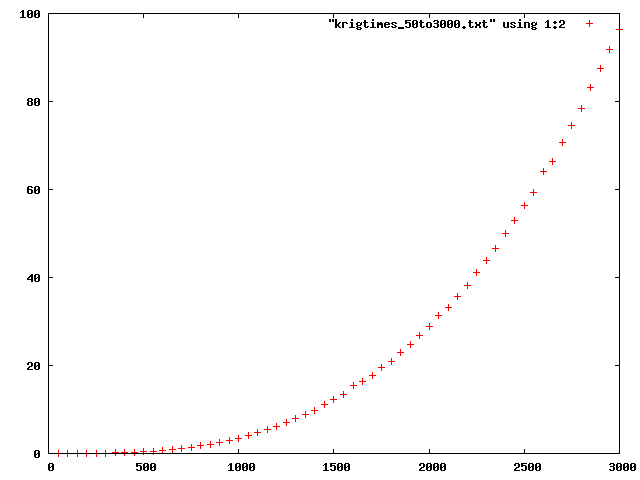
\includegraphics[width=12cm]{kriging_times_50to3000.png}
\end{figure}

We will use Surfpack to generate an empirical model from these data, which we can then use to predict running times on problem sizes for which we have not gathered actual data.

Parts of the data file are shown in figure xx.
\verbatiminput{sampledata.txt} 

This data includes problems using up to 3000 points (which requires the inversion of a 3000 by 3000 matrix).  After we create a model to fit these data, we will evaluate the model to predict running times for problems with up to 5000 points.

The first step is to load the data from the file.

\texttt{LoadData[name = timing\_data, file = 'krigtimes\_50to3000.txt']}

From the plot of the data, we can see that the trend in the data is definitely not linear.  We will attempt to fit the data using a quadratic polynomial.

\texttt{CreateSurface[name = poly2, data = timing\_data, type = polynomial, order =2 ]}

We can use Surfpack to generate the set of test data points and then evaluate the model on those data. 
\verbatiminput{timingdataevalandsave.spk}

Figure xxx shows a portion of the output file test\_timing\_data.txt, which lists the predictions of the model for problem sizes of 50 to 5000, at 50 point intervals.

\verbatiminput{testtimingdatasnippet.txt}

A plot of the observed data and model predictions is shown in figure xxx.

\begin{figure}[htbp]
\includegraphics[width=12cm]{quad_poly.png}
\end{figure}

Figure xxx shows an excerpt from quad\_poly\_snippet.txt, which shows the formula for the quadratic approximation.

\verbatiminput{quadpolysnippet.txt}

\[ time = \hat{f}(numpts) \approx 1.62x^2 - 0.02x + 5.14 \]

The predictions appear to follow the general trend of the data fairly well.  The model does curve away from the observed values at the lower-valued data points, but we are more likely to be concerned about the predictions for larger-sized problems.

We can use Surfpack's Fitness command to quantify the error between the model and the data.  We will use the mean\_abs metric as an example, which computes the absolute value of the difference between each data point used to create the model and the prediction of the model at that point.  The reported value is the mean of those residuals.

\texttt{mean\_abs for poly2: 1.48252}

The value of 1.48 means that, on average, the predicted running time differs from the reported running time by 1.48 seconds.  The shape of the data and/or knowledge of the underlying matrix inversion algorithm may suggest to us that a cubic polynomial would provide a better fit here.

Two other common goodness-of-fit metrics are PRESS and R-Squared.

\verbatiminput{pressandrsquaredresults.txt}
PRESS gives an average for what the error would be at each data point, if that point were not included in building the model.  Values close to zero are more desirable.  The R-Squared metric measures the fraction of variance in the model that can be attributed to the variance in the data.  Values close to 1 are more desirable.

The plots of the data and/or knowledge of the underlying matrix inversion algorithm may motivate us to try to fit a cubic polynomial to the data.

\verbatiminput{cubic_poly.spk}

All of the metrics are worse; this raises some red flags.  In particular, it is not possible for the R-Squared value to be lower for a least-squares fit to a cubic polynomial than for a quadratic.

The file cubicpolytiming.txt shows the coefficients for the model.

\verbatiminput{cubicpolytiming.txt}


\[ time = \hat{f}(numpts) \approx - 0.0007x + 0.1095 \]

The cause of the problem is matrix ill-conditioning.  The range of the problem sizes is 50--3000, while the running times range from a fraction of a second up to about 100 seconds.  To address this problem, we scale the data so that data fall in the range from 0--1.

\verbatiminput{scaledcubic.spk}

(Include plot)

Now all the metrics are improvements over the quadratic fit, which suggests that the cubic-polynomial more accurately reflects the trends in the data.  In the absence of any additional information, we would likely use the cubic-polynomial model to make predictions about running times. 

Suppose there were computational resources available to generate a few more data points.  Running times for problem sizes of 3050--5000 points are given in the file test\_times.txt.  Now we can evaluate our quadratic and cubic models on these new data and get a better comparison of their predictive capabilities.

\verbatiminput{timing3050.txt}

\begin{centering}
\begin{figure}[htbp]
\includegraphics[width=12cm]{quad_poly_0to5000_with_pred.png}
\end{figure}
\end{centering}

The predictions for the cubic-polynomial are truly impressive.  For a problem sizeof 5000, the true running time was 437 seconds and the prediction was 439 seconds.
\subsection{Topology }
\verbatiminput{marskrig.spk}
\verbatiminput{marskrig.results}

\subsection{Rosenbrock}
%
%\section{Data-fitting algorithms}
%\subsection{Least-squares Polynomial Regression}
%\subsection{Multivariate Adaptive Regression Splines (MARS)}
%\subsection{Kriging Interpolation}
%\subsection{Radial Basis Functions}
%\subsection{Artificial Neural Network}
%
%\section{Fitness metrics}
%
%\section{Test Functions}
%
%\section{Surfpack Library API}
%Brief explanation for writing custom C++ code and linking against the Surfpack library.
%
%\section{Extending Surfpack}
%\subsection{Adding a new surface method}
%\subsection{Adding a goodness-of-fit metric}
%\subsection{Adding a new command-line option}
%
%\section{Using Surfpack with Dakota}
%Brief explanation of how Surfpack fits in with Dakota.  Pointer to Dakota manuals for detailed information about accessing the various options.
%
\section{Troubleshooting}
List of error messages with probable causes and suggestions for resolving them.

\subsubsection{Bad surface name in file}
When a surface object is read in from a file, the first item listed should be the name of the surface type (Polynomial, Kriging, etc.) Check to make sure that the file being read in is indeed a surface file and that it has a valid type identifier.  

\subsubsection{Cannot add another response: the number of new response values does not match the size of the physical data set.}
This happens when some of the points in a data set have been designated as "excluded."  A list of new response values cannot be added in this state, because if the currently excluded points were to be included again, they would not have a needed value for the new response.  Future releases will support multi-response data setsin which values for some responses may be missing.

To circumvent this problem, activate all points prior to adding a response, or copy the active points into a new SurfData object, and add the response to the new set.


\subsubsection{Cannot add response because there are no data points}
The SurfData object to which an attempt is being made to add response data contains no data points.  The number of points in the data set should correspond to the number of new response values being added.

\subsubsection{Cannot compute euclidean distance. Vectors have different sizes.}
When computing the distance between two vectors, v1 and v2, make sure that v1.size() == v2.size().

\subsubsection{Cannot create surface with zero dimensionality}
A query has been made to Polynomial::minPointsRequired in which the dimensionality of the data set has been declared to be zero.  All data sets must have dimensionality of at least one.

\subsubsection{Cannot set response index on NULL data }
A response\_index argument has been passed to a Surface object for which the data set has not yet been specified.  First, specify the data set, using either the constructor or the setData method.  Then call the config method with an response\_index Arg object that specifies which response value will be used to create the surface.

\subsubsection{Cannot specify both data and surface.}
The Save command can be used to write either a data object or a surface object to a file, but not both.  Specify one or the other.  If both a surface and a data set need to be saved, use two Save commands.

\subsubsection{Data variable not found in symbol table}
The variable name given for the data argument in a CreateSurface, Fitness, or Evaluate command was not found in the symbol table.  Make sure that the data object of that name was previously loaded from a file or created using a GridPoints or MonteCarloSample command.  Check for misspellings.

\subsubsection{Data unacceptable: there is no data.}
An attempt was made to create a Surface object without specifying any data.  Pass data into the Surface object through the constructor or through the setData method before invoking createModel.

\subsubsection{Axes variable not found in symbol table.}
The variable name given for the axes argument in a GridPoints or MonteCarloSample command was not found in the symbol table.  Make sure that the axes object of that name was previously loaded from a file or created using a CreateAxes command.  Check for misspellings.

\subsubsection{Dimensionality of data needed to determine number of required samples.}
This error occurs when a request is made to know the minimum number of required sample for some surfaces before the dimensionality of the data is determined.  In many cases the required number of points is a function of the arity of the data.

\subsubsection{Dimension mismatch: conmin seed and data dimensionality.}
By default the correlation parameters for Kriging are computed using doing a maximum likelihood estimation.  If a seed for the optimization is specified, it should be a tuple with the same dimensionality as the data set.

\subsubsection{Dimension mismatch: correlations and data dimensionality}
Kriging expects one correlation value per dimension in the data set.

\subsubsection{Dim mismatch in SurfData::setFLabels}
The wrong number of labels was given for the data set.  These labels are only for the response variables.  Use setXLabels to specify tags for the predictor variables.

\subsubsection{Dim mismatch in SurfData::setXLabels}
The wrong number of labels was given for the data set.  These labels are only for the predictor variables.  Use setFLabels to specify tags for the response variables.

\subsubsection{End of file reached unexpectedly.}
When reading data in from a file, there were fewer points than expected in the file or fewer values for a particular point than were expected.  Please check the data file.

\subsubsection{Error in dgglse}
The info flag to the LAPACK routine dgglse returned a non-zero value.  See the LAPACK documentation for details.  The dgglse routine is used in conjunction with constrained least-squares solves in the PolynomialSurface class.

\subsubsection{Cannot add response because physical set size is different than logical set size.}
Before adding another response, clear excluded points or create a new data set by using the SurfData::copyActive method.  This inconvenience will be resolved in future releases.

\subsubsection{Cannot write SurfData object to stream.  No active data points.}
Clear the excluded data points before writing the data to a file.

\subsubsection{Data unacceptable: this surface requires....} 
The various data-fitting algorithms have their own requirements for how many points are necessary to compute an approximation.  Use the numPointsRequired method to find how many points are required.  Note that this is only the minimum number of points for the algorithm to perform its computations.  The number of points needed to get a model that gives useful predictions may be much, much greater.  Quantifying these needs is the subject of current research.

\subsubsection{Error in SurfData::addPoint. Points in this data set have....}
The collection of points in a SurfData object must all have the same number of predictor variables.  Currently, they must also have the same set of response variables, although this requirement will be relaxed in future releases.

\subsubsection{Error in SurfData::sanityCheck....} 
Surfpack has discovered a mismatch in the dimensionality of at least two data points in a single SurfData object.  This error can be caused by the modification of individual SurfPoint objects (through external handles) after they have been added to a SurfData object.  While there are legitimate uses of external handles to a SurfData object's data points, care must be taken to avoid this kind of inconsistency.

\subsubsection{Requested ... max index ....}
A data point was requested from a SurfData object, but the index given is equal to or greater than the number of points in the set.  Remember that if there are $n$ points, the indices from those points are $0, 1, \ldots, n-1$.

\subsubsection{Exception caught and rethrown in SurfPoint::readText}
\subsubsection{Exception rethrown in SurfPoint::readBinary}
An unknown error occured while reading a file.  Check the integrity of your data.

\subsubsection{Expected: \ldots found: \ldots} 
The name found in a surface file is inconsistent with the type of Surface object that is being create from the file.  Check the file contents and object constructor.

\subsubsection{Expected `f' or `v' on line}
The first line of an axes object should be the number of dimensions desired in theresulting data set.  Each line after the first should either give a minimum, maximum, and number of raster points for one dimension, or it should give a fixed valuefor a dimension, which all points in the set will share.  Lines with fixed values should begin with the flag `f'; all others should begin with `v' (for `variable').
\subsubsection{Index \ldots specified, but there are zero\ldots}
Either a request has been made for a data point in a data set where there are no active points, or a request has been made for a non-existent response variable.  Remember the if there are $n$ response variables, they are indexed from $0$ to $n-1$.  When requesting data points from a SurfData object, remember that some points may be inactive (excluded), which would reduce the maximum valid index.

\subsubsection{In Surface::checkData: No data was passed in}
Data for a surface may be specified in the constructor of a Surface object, or using the setData method.  If neither of these things occurs before the createModel method is invoked (either directly or indirectly), this error could result.

\subsubsection{Integer overflow: number of terms exceeds maximum integer}
There are too many terms in the regression model.  Use a lower-order polynomial to fit the data or project the data into a lower-dimensional space.

\subsubsection{Must know data arity to use uniform correlation value.}
Kriging allows for the specification that the same correlation parameter should be used for each dimension, but the number of dimensions must be known in advance.  Specify the data for the KrigingSurface object before invoking this method.

\subsubsection{Expected on this line\ldots}
The number of predictor and/or response variables on some line in the data file does not match the specified number(s) for the file.  Check the format of the file.

\subsubsection{No axes argument specified.}
A GridPoints or MonteCarloSample command was given, but no axes variable was specified.  The axes variable must be created in a previous command.  It specifies the (hypercube) boundaries for the data set, and in the case of the GridPoints command, the number of raster points per dimension.

\subsubsection{No data argument specified.}
A data argument is required for the CreateSurface and Evaluate commands.  The data object must have been created (and named) previously in a LoadData, GridPoints, or MonteCarloSample command.

\subsubsection{No error metric of that type in this class.}
Not all metrics are supported by all methods.  Consider using an alternate metric or extending Surfpack to support the desired metric.

\subsubsection{No existing surface variable specified.}
The Fitness command requires the name of a Surface object that has already been created by a LoadSurface or CreateSurface command.

\subsubsection{No filename specified.}
All of the Load and Save commands require a valid file name to be given.  In all cases, the name of the appropriate argument is `file'.

\subsubsection{No fitness metric specified.}
The Fitness command requires the specification of a metric.  See section xx for a discussion of supported metrics.  See section xx for an explanation of how to extend Surfpack with a new metric.  In arguments to the Fitness command, names of metrics should not be quoted.
\subsubsection{No name argument specified.}
The LoadData, LoadSurface, CreateAxes, CreateSurface, GridPoints, and MonteCarloSample all create new objects that are to be stored in the symbol table for future reference.  Each command requires a name argument that gives a designation to the new entity.

\subsubsection{No surface or data argument specified.}
The Save command expects either a surface argument or a data argument (but not both).  Check for misspellings.

\subsubsection{No surface type specified.}
The CreateSurface command requires a type argument to specify which algorithm should be used to approximate the data: polynomial, kriging, mars, ann, or rbf.  See section xx for an explanation of these algorithms.

\subsubsection{Not enough data to compute PRESS.}
If a Surface object is created using the minimum number of required samples, then the PRESS error metric may not be computed.  PRESS creates the $n$ additional models using the same algorithm, but excluding one of the given points each time and then predicting the value of that point after the model has been created.  However, if leaving one point out causes the amount of available data to fall below what is required, there is no way to compute the metric. 

\subsubsection{Out of range in SurfPoint}
The $i$th dimension was requested, but the data has $i$ or fewer dimensions.  Remember that if the data has $n$ dimensions, they are indexed from 0 to $n-1$.

\subsubsection{Size of set of excluded points exceeds size of SurfPoint set}
Some of the indices passed in to setExcludedPoints must either be out of the range of acceptable indices for the data set, or duplicatations of other excluded points.

% Surface name not found.
\subsubsection{Surface variable not found in symbol table}
The variable name given for the surface argument in a Fitness or Evaluate command was not found in the symbol table.  Make sure that the surface object of that name was previously loaded from a file or created using a LoadSurface or CreateSurface command.  Check for misspellings.
\subsubsection{There are no response values associated with this point}
A response value has been requested for a data point for which there are no responses.  If the data were read in from a file, check to make sure the contents of the file are as expected.

\subsubsection{This Rval class does not have such a value}
This error generally means that the type of an argument in a Surfpack command was different than what was expected.  Common mistakes are using quoted string literals where unquoted identifiers are expected (or vice versa), or specifying a single item when a tuple (a parenthesized list of values) is expected.

\subsubsection{Unrecognized filename extension.  Use .sd or .txt}
\subsubsection{ Unrecognized filename extension.  Use .srf or .txt}
Surfpack uses file extensions to determine the formatting of information that is read from or written to files.  Currently all Data and Surface files should have a txt extension.  Future releases will support a binary format for both data and surfaces.  The binary formats will be more compact and will provide better I/O performance for large data sets.

% Unrecognized option for surface parameter 'scaling'
\appendix

\begin{sidewaystable}[h]
  \centering
  \begin{tabular}{|c|c|c|c|c|}
    \hline
    \textbf{Command} & \textbf{Argument} & \textbf{Type} &
    \textbf{Req.} & \textbf{Meaning}\\
    \hline
    CreateAxes & name & identifier & yes & Variable name by which
    this definition can be referred to in later commands.\\
    \hline
    & file & string & yes & File to be read.\\
    \hline
    CreateSurface & name & identifier & yes & Variable name by which
    this surface can be referred to in later commands.\\
    \hline
    & type & identifier & yes & Must be one of ann, mars, kriging, polynomial,
    or rbf.\\
    \hline
    & data & identifier & yes & Name of the data set used to
    build surface.\\
    \hline
    & response\_index & integer & no & Specifies which response
    should be used to create this surface.\\
    & & & & The default value is 0 (i.e., the first response value
    listed).\\
    \hline
    Evaluate & surface & identifier & yes & The name of the surface to
    be evaluated.\\
    & & & & Must have been created or loaded in a previous command.\\
    \hline
    & data & identifier & yes & Data set that the surface is to
    be evaluated on.  Must have been created  \\
    & & & & or loaded in a previous command.  In absensce of 'name' argument,\\
    & & & & results are appended to this data as a new response variable. \\
    \hline
    & name & identifier & no & Name of a new data set, to which the results\\
    & & & & will be appended as the first response variable. \\
    & & & & It must NOT be the name of a data set that was created or
    loaded\\
    & & & & in a previous command.\\
    \hline
    Fitness & surface & identifier & yes & Name of surface to be
    evaluated.\\
    \hline
    & metric & identifier & yes & Must be one of press, rsquared,
    mean\_squared, sum\_squared, max\_squared, \\ 
    & & & & mean\_scaled, sum\_scaled, max\_scaled, mean\_abs, sum\_abs, \\
    & & & & max\_abs, mean\_relative, max\_relative, root\_mean\_squared.\\
    \hline
    & data & identifier & no & The data used to compute the metric.
    If not specified, the default\\
    & & & & is to use the same data that were used to build the
    surface.\\
    \hline
    & response\_index & integer & no & Specifies which response
    variable in the data\\ & & & & set should be used as the ``true'' value when the\\
    & & & & fitness of the surface is being computed.\\
    \hline
    GridPoints & name & identifier & yes & Variable name by which the
    resulting data set can be referred to in later commands.\\
    \hline
    & axes & identifier & yes & Axes variable that specifies the
    boundaries\\
    & & & & and number of points along each dimension.\\
    \hline
    & test\_function & identifier & no & Name of a test function to add on
    as a response variable for this data.\\
    & & & & Must be one of `rosenbrock', `rastrigin', `quasisine',
    `shpere' or `sumofall'.\\
    & & & & Multiple test\_function arguments may be included in a
    single command.\\
    \hline
    LoadData & name & identifier & yes & Variable name by which this
    data can be referred to in later commands.\\
    \hline
    & file & string & yes & Name of file to be read.\\
    & & & & Must have .txt extension.\\
    \hline
    LoadSurface & name & identifier & yes & Name by which
    this surface variable can be referred to in later commands.\\
    \hline
    & file & string & yes & Name of file to be read.  Must have .txt
    extension.\\
    \hline
    MonteCarloSample & name & identifier & yes & Name by
    which the resulting data set can be referred to in later commands.\\
    \hline
    & axes & identifier & yes & Axes variable that specifies the
    boundaries along each dimension.\\
    & & & & Must have been created in a previous command.\\
    \hline
    & test\_function & identifier & no & Same as for the
    GirdPoints command.\\
    \hline
    & size & integer & no & Number of random samples.  Default is
    100.\\
    \hline
    Save & surface/data & identifier & yes & Name of data or
    surface to be saved.  Must have been previously defined.\\
    \hline
    & file & string & yes & Name of file to be written to.  Must have .txt
    extension.\\
    \hline
  \end{tabular}
  \caption{\textbf{Surfpack Command Summary}}
\end{sidewaystable}

\begin{sidewaystable}
  \centering
  \begin{tabular}{|l|l|l|l|l|l|}
    \hline
    \textbf{Argument} & \textbf{For} & \textbf{Type} & \textbf{Req.} &
    \textbf{Default} & \textbf{Meaning}\\
    \hline
    order & polynomial & integer & no & 2 & Maximum order of
    polynomial regression.\\
    \hline
    norm\_bound & ann & real & no & 0.8 & ?\\
    \hline
    svdfactor & ann & real & no & 0.9 & Range 0-1.\\
    \hline
    fraction\_withheld & ann & real & no & 0.0 & Fraction of data set
    used for validation.\\
    \hline
    conmin\_seed & kriging & tuple & no & (1.0,\ldots,1.0) & Initial
    values of correlation parameters passed to conmin optimizer.\\
    & & & & & The tuple (vector must have the same dimensionality as
    the data set.\\
    \hline
    theta\_vars & kriging & tuple & no & conmin & Exact correlation
    parameters to be used.  If theta\_vars are specified,\\
    & & & & & conmin is bypassed altogether.  The tuple (vector)
    must have the\\
    & & & & & same dimensionality as the data set.\\
    \hline
    max\_bases & mars & integer & no & 25 & Maximum number of basis
    functions.\\
    \hline
    max\_interactions & mars & integer & no & 2 & Maximum number of
    varaible interactions that will be considered.\\
    \hline
    interpolation & mars & string & no & `cubic' & Must be either
    `linear' or `cubic'.  Determines what kind of splines\\
    & & & & & are used after surface is built.\\
    \hline
    radius & rbf & real & no & 0.1 & Radius of the basis
    functions.\\
    \hline
  \end{tabular}
  \caption{\textbf{Surface Method Argument Summary}}
\end{sidewaystable}

\end{document}
 
